\documentclass[10pt]{article}
\usepackage{icmlko}

\icmlmeta{IP 파운데이션 월드모델}{12}{분산은 증폭기다}{노트 11의 원리를 일반화하려다 절반을 철회한다 --- 분산은 옳은 계수를 키우고 틀린 계수도 키운다}

\begin{document}

\twocolumn[
\icmlheader

\begin{abstract}
노트 11은 굿즈 규모 축 하나에서 ``축은 그 모집단에서 변해야 예측할 수 있다''를 관측하고
일반 원리로 제시했다. 같은 노트에 반증 조건도 적었다 --- 다른 축에서도 같은 패턴이
보여야 하며, 그렇지 않으면 이 축 하나의 우연이라고. 두 도메인 $\times$ 세 축 $\times$
여러 시기로 24개 셀을 만들어 검정했다. \textbf{일반화되지 않는다.} 전체 셀에서
축 표준편차와 예측 성적의 상관은 $-$0.03(스피어만 $-$0.21, p=0.45)로 사실상 없다.
그런데 축별로 쪼개면 부호가 갈린다 --- 전이가 확인된 굿즈 규모는 $-$0.45, 전이되지
않는 두 축은 $+$0.43이다. 이것이 정제된 가설을 낳는다. \textbf{분산은 축의 예측력을
만드는 것이 아니라 계수가 하는 일을 증폭한다.} 계수가 옳으면 분산이 클수록 좋아지고,
틀리면 분산이 클수록 나빠진다. 다만 이 가설도 확정하지 못한다 --- 두 집단의 상관
격차 $-$0.878에 대한 순열 검정이 p=0.11이다. 그리고 방법론적 교훈이 하나 더 있다.
굵은 구간으로 셀 5개를 만들었을 때 굿즈 규모의 상관은 $-$0.924였는데 세분해 8개로
만들자 $-$0.451이 됐다. \textbf{셀을 어떻게 나누느냐가 상관의 크기를 절반으로 바꾼다.}
노트 11의 실무 권고 --- 라벨 없이 분산만 보고 적용 가능성을 판정한다 --- 도 철회한다.
\end{abstract}
]

\section{반증 조건을 실행했다}

노트 11의 주장 상자는 이랬다.

\begin{quote}\fontsize{9.2}{11}\selectfont
축의 예측력은 그 축이 대상 모집단에서 얼마나 변하는가에 달려 있다. 도메인 불변성과는
별개의 조건이다 --- 계수가 옳아도 축이 상수면 쓸모가 없다.\\[0.3em]
\textbf{반증 조건.} 다른 축에서도 같은 패턴이 보여야 한다. 축의 구간 내 표준편차와
그 구간의 전이 성적이 상관되지 않으면 이 설명은 이 축 하나에만 해당하는 우연이다.
\end{quote}

설계는 단순하다. 두 도메인(팝업, 아이돌) $\times$ 세 축(타깃 폭, 미디어 투입,
굿즈 규모) $\times$ 여러 시기로 셀을 만들고, 각 셀에서 축의 표준편차와 예측 성적을
잰다. 셀 안에서 학습하지 않고 \emph{상대 도메인 전체에서 배운 계수}를 그대로
적용한다 --- 셀 안에서 학습하면 분산이 작을 때 과적합으로 오히려 좋아 보인다.

\section{일반화되지 않는다}

\begin{table}[t]
\centering\tsize
\caption{전체 셀에서 축 표준편차와 예측 성적의 상관.}
\begin{tabular}{lrr}
\toprule
분할 & 셀 & 스피어만 $\rho$ \\
\midrule
굵은 구간 (3구간) & 15 & $-$0.211 (p=0.45) \\
세분 구간 (6구간) & 24 & --- \\
\bottomrule
\end{tabular}
\end{table}

전체를 뭉쳐 보면 관계가 없다. 노트 11의 주장을 일반 원리로 유지할 수 없다.

\claimx{노트 11의 ``축은 변해야 쓸모가 있다''를 일반 원리로 제시한 것을 철회한다.
두 도메인 세 축 스물네 셀에서 축 표준편차와 예측 성적은 상관되지 않는다.}{셀을
훨씬 많이 만들 수 있는 규모에서 상관이 살아나면 철회가 성급했던 것이다.}

\section{그런데 부호가 축마다 갈린다}

뭉치면 사라지지만 쪼개면 선명하다.

\begin{figure}[t]
\centering
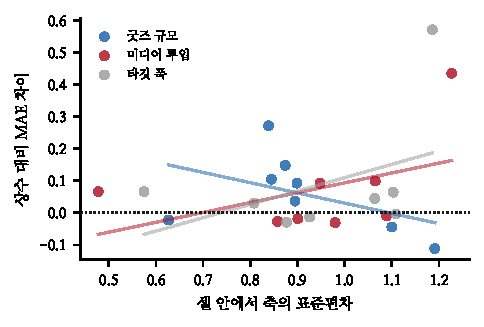
\includegraphics[width=\columnwidth]{figs/scatter.pdf}
\caption{셀별 축 표준편차와 예측 성적. 굿즈 규모만 기울기가 음이고 나머지 둘은
양이다. 선은 각 축의 최소제곱 적합.}
\end{figure}

\begin{table}[t]
\centering\tsize
\caption{축별 상관(세분 구간, 축마다 셀 8개). 전이 여부는 노트 10의 결과다.}
\begin{tabular}{lrrl}
\toprule
축 & 피어슨 & 스피어만 & 전이 여부 \\
\midrule
굿즈 규모   & $-$0.451 & $-$0.595 & 전이됨 (p=0.034) \\
미디어 투입 & $+$0.440 & $+$0.452 & 약함 (39\%) \\
타깃 폭     & $+$0.425 & $+$0.238 & 안 됨 (10\%) \\
\bottomrule
\end{tabular}
\end{table}

전이가 확인된 축만 음의 기울기를 갖는다. 전이되지 않는 두 축은 양의 기울기다 ---
\emph{분산이 클수록 더 나빠진다.}

이 패턴은 해석이 자연스럽다. 예측값은 계수와 축 값의 곱이다. 축이 변하지 않으면
예측도 변하지 않으므로 계수가 옳든 그르든 상수 예측기와 다르지 않다. 축이 크게
변하면 예측도 크게 변한다 --- 계수가 옳으면 옳은 방향으로, 틀리면 틀린 방향으로.

\claimx{분산은 축의 예측력을 만드는 것이 아니라 계수가 하는 일을 증폭한다.
옳은 계수에는 이득이고 틀린 계수에는 해악이다.}{전이가 확인된 축에서 분산이 클수록
나빠지는 셀이 다수 나오면 증폭 해석이 틀린 것이다.}

\subsection{그러나 확정하지 못한다}

두 집단(굿즈 규모 대 나머지)의 상관 격차를 순열 검정했다. 셀에 붙은 축 이름을
20,000회 섞어 귀무 분포를 만들었다.

\begin{figure}[t]
\centering

\includegraphics[width=\columnwidth]{figs/perm.pdf}
\caption{축 이름을 섞었을 때의 상관 격차 분포와 관측값. 관측 격차는 크지만
귀무 분포도 넓다.}
\end{figure}

\begin{table}[t]
\centering\tsize
\caption{상관 격차의 순열 검정. 셀 24개, 20,000회.}
\begin{tabular}{lr}
\toprule
굿즈 규모 상관 & $-$0.451 \\
나머지 두 축 상관 & $+$0.427 \\
격차 & $-$0.878 \\
순열 p & \textbf{0.111} \\
\bottomrule
\end{tabular}
\end{table}

격차는 크지만 p=0.111이다. 셀이 24개뿐이고 축이 셋뿐이라 검정력이 없다. 증폭 가설은
\textbf{그럴듯하나 확정되지 않은} 상태로 남긴다.

\section{셀을 나누는 방식이 결론을 바꾼다}

한 가지 더 기록해 둘 것이 있다. 처음에 세 구간으로 굵게 나눴을 때 굿즈 규모의
상관은 $-$0.924였다. 여섯 구간으로 세분하자 $-$0.451이 됐다. 같은 데이터, 같은 축,
절반으로 줄어든 상관이다.

\begin{figure}[t]
\centering
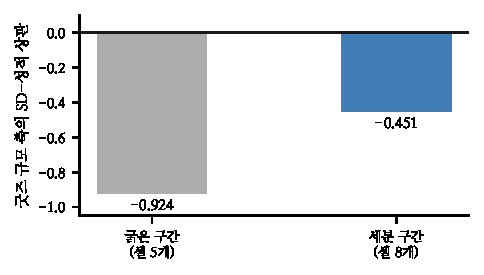
\includegraphics[width=\columnwidth]{figs/cells.pdf}
\caption{셀을 어떻게 나누느냐가 상관의 크기를 절반으로 바꾼다. 왼쪽 값을 보고
``원리를 확인했다''고 썼다면 과대주장이었다.}
\end{figure}

굵은 구간에서는 셀이 다섯 개뿐이고 각 셀이 크므로 셀 내부 잡음이 평균되어 점들이
매끈하게 늘어선다. 세분하면 셀마다 표본이 작아져 점이 흩어진다. 어느 쪽이 옳은
숫자인가 --- 둘 다 같은 관계의 다른 해상도이며, \emph{높은 상관이 강한 증거라고
읽으면 안 된다}는 것이 요점이다.

노트 7에서 ``폴드 넷으로는 부호도 정하지 못한다''고 썼는데, 같은 병이 여기서는
셀 개수로 나타났다. 집계 단위를 크게 잡으면 상관이 커진다는 것은 생태학적 오류의
고전적 형태다.

\claimx{집계 단위를 크게 잡을수록 상관이 커진다. 셀 개수를 함께 보고하지 않은
상관계수는 해석할 수 없다.}{셀 크기를 바꿔도 상관이 유지되는 관계가 있다면 그것은
집계 수준에 무관한 진짜 관계다. 이 데이터에서는 그런 것을 아직 못 찾았다.}

\section{실무 권고를 철회한다}

노트 11은 이렇게 썼다.

\begin{quote}\fontsize{9.2}{11}\selectfont
셋째 조건은 사전에 라벨 없이 확인할 수 있다는 장점이 있다. 축 값만 재보면 되기
때문이다. 적용 가능성 점검의 첫 관문으로 쓸 수 있다.
\end{quote}

이 권고를 철회한다. 분산이 크다는 것은 축이 \emph{무언가를 크게 할 것}이라는 뜻일 뿐
그것이 이득인지 해악인지 말해 주지 않는다. 전이되지 않는 두 축에서는 분산이 클수록
성적이 나빠졌다. 라벨 없이 판정할 수 있다는 부분이 틀렸다 --- 계수의 타당성을 먼저
확인해야 하고, 그것은 라벨을 요구한다.

적용 가능성 점검의 순서는 이렇게 고친다.

\begin{enumerate}[leftmargin=1.3em,itemsep=0.15em]
\item 이 도메인에서 축이 같은 부호로 작동하는가 --- \emph{라벨 필요} (노트 9--10).
\item 축 측정의 신뢰도가 문턱을 넘는가 --- \emph{라벨 필요} (노트 9, r$\geq$0.79).
\item 계수가 확인된 뒤에, 이 모집단에서 축이 충분히 변하는가 --- 라벨 불필요.
\end{enumerate}

셋째는 여전히 유용하지만 \emph{첫째와 둘째 뒤에} 온다. 순서가 뒤바뀌면 틀린 계수를
증폭할 모집단을 골라 놓고 잘 될 것이라 기대하게 된다.

\section{한계}

\begin{itemize}[leftmargin=1.1em,itemsep=0.15em]
\item 셀 24개, 축 3개. 순열 검정의 검정력이 낮다.
\item 전이 여부를 노트 10에서 가져와 축을 두 집단으로 나눴는데, 그 판정 자체가
      같은 데이터에서 나왔다. 완전히 독립적인 분류가 아니다.
\item 시기 구간은 데뷔 연도만 썼다. 다른 분할(카테고리, 소속사 규모)에서도
      같은 패턴인지 보지 않았다.
\item 팝업 쪽은 2022년 이전 표본이 적어 구간이 둘뿐이다.
\end{itemize}

\section{다음}

\begin{enumerate}[leftmargin=1.3em,itemsep=0.15em]
\item 세 번째 도메인 확보 --- 축을 늘리는 것보다 도메인을 늘리는 것이 셀을 빨리
      늘린다. 증폭 가설의 검정력도 거기서 나온다.
\item 아이돌 굿즈 규모 사람 태깅과 신뢰도 측정 --- 노트 10의 비대칭 설명 검정.
\item 카테고리·소속사 규모 분할에서 증폭 패턴 재확인.
\item 새 타깃 폭으로 아이돌 축 갱신 후 전이 재검정.
\end{enumerate}

\vspace{0.6em}
\hrule height 0.3pt
\vspace{0.5em}
{\footnotesize
\textbf{참고문헌}\\[0.3em]
Good, P. (2005). \emph{Permutation, Parametric, and Bootstrap Tests of Hypotheses},
3rd ed. Springer.\\[0.15em]
Robinson, W. S. (1950). Ecological correlations and the behavior of individuals.
\emph{American Sociological Review}, 15(3), 351--357.\\[0.15em]
Openshaw, S. (1984). \emph{The Modifiable Areal Unit Problem}. Geo Books.\\[0.15em]
Carroll, R. J. et al. (2006). \emph{Measurement Error in Nonlinear Models},
2nd ed. Chapman \& Hall.
}

\end{document}
